\chapter{Experiment setups}
\indent
    Experiment setups are listed in this chapter including 7 parts, 
    encoder, decoder, prior model (including re-parameterization trick), predictor model, data loader, KL annealing, and teacher-forcing.

\section{Encoder}
\indent
	Encoder encodes input frames as latent vector. \\
    In this experiment, encoder is implemented by VGG (See Listing \ref{encoder}).

\begin{lstlisting}[language=Python, caption={Python code of \textcolor{blue}{\textbf{VggEncoder}}.}, label={encoder}]
class VggEncoder(nn.Module):
    def __init__(self, dim: int) -> None:
        super().__init__()
        
        self.dim = dim
        
        # 64 x 64
        self.c1 = nn.Sequential(
            VggLayer(3, 64),
            VggLayer(64, 64),
        )
        # 32 x 32
        self.c2 = nn.Sequential(
            VggLayer(64, 128),
            VggLayer(128, 128),
        )
        # 16 x 16 
        self.c3 = nn.Sequential(
            VggLayer(128, 256),
            VggLayer(256, 256),
            VggLayer(256, 256),
        )
        # 8 x 8
        self.c4 = nn.Sequential(
            VggLayer(256, 512),
            VggLayer(512, 512),
            VggLayer(512, 512),
        )
        # 4 x 4
        self.c5 = nn.Sequential(
            nn.Conv2d(512, dim, 4, 1, 0),
            nn.BatchNorm2d(dim),
            nn.Tanh()
        )
        self.mp = nn.MaxPool2d(
            kernel_size=2, stride=2, padding=0)

    def forward(self, input: torch.FloatTensor) -> torch.FloatTensor:
        h1 = self.c1(input) # 64 -> 32
        h2 = self.c2(self.mp(h1)) # 32 -> 16
        h3 = self.c3(self.mp(h2)) # 16 -> 8
        h4 = self.c4(self.mp(h3)) # 8 -> 4
        h5 = self.c5(self.mp(h4)) # 4 -> 1
        
        return h5.view(-1, self.dim), [h1, h2, h3, h4]\end{lstlisting}

\section{Decoder}
\indent
    Decoder decodes output from encoder and fixed prior model, 
    and gets next predicted frame. \\
    In this experiment, decoder is implemented by VGG (See Listing \ref{decoder}).

\begin{lstlisting}[language=Python, caption={Python code of \textcolor{blue}{\textbf{VggDecoder}}.}, label={decoder}]
class VggDecoder(nn.Module):
    def __init__(self, dim: int) -> None:
        super().__init__()
        
        self.dim = dim
        
        # 1 x 1 -> 4 x 4
        self.upc1 = nn.Sequential(
            nn.ConvTranspose2d(dim, 512, 4, 1, 0),
            nn.BatchNorm2d(512),
            nn.LeakyReLU(0.2, inplace=True)
        )
        # 8 x 8
        self.upc2 = nn.Sequential(
            VggLayer(512 * 2, 512),
            VggLayer(512, 512),
            VggLayer(512, 256)
        )
        # 16 x 16
        self.upc3 = nn.Sequential(
            VggLayer(256 * 2, 256),
            VggLayer(256, 256),
            VggLayer(256, 128)
        )
        # 32 x 32
        self.upc4 = nn.Sequential(
            VggLayer(128 * 2, 128),
            VggLayer(128, 64)
        )
        # 64 x 64
        self.upc5 = nn.Sequential(
            VggLayer(64 * 2, 64),
            nn.ConvTranspose2d(64, 3, 3, 1, 1),
            nn.Sigmoid()
        )
        self.up = nn.UpsamplingNearest2d(scale_factor=2)

    def forward(self, input: torch.FloatTensor) -> torch.FloatTensor:
        vec, skip = input 
        
        d1 = self.upc1(vec.view(-1, self.dim, 1, 1)) # 1 -> 4
        up1 = self.up(d1) # 4 -> 8
        d2 = self.upc2(torch.cat([up1, skip[3]], 1)) # 8 x 8
        up2 = self.up(d2) # 8 -> 16 
        d3 = self.upc3(torch.cat([up2, skip[2]], 1)) # 16 x 16 
        up3 = self.up(d3) # 8 -> 32 
        d4 = self.upc4(torch.cat([up3, skip[1]], 1)) # 32 x 32
        up4 = self.up(d4) # 32 -> 64
        
        output = self.upc5(torch.cat([up4, skip[0]], 1)) # 64 x 64
        
        return output\end{lstlisting}

\section{Prior model}
\indent
    Prior model gets encoder output as its input, 
    and outputs mean and log variance (to ensure positive standard deviation). 
    Then, use re-parameterization trick to make gradient being successfully back-propagated. \\
    In this experiment, decoder is implemented by LSTM (See Listing \ref{prior}).

\begin{lstlisting}[language=Python, caption={Python code of \textcolor{blue}{\textbf{GaussianLstm}} (some code is omitted).}, label={prior}]
class GaussianLstm(nn.Module):
    def __init__(self, 
            input_size: int, output_size: int, hidden_size: int, num_layers: int, 
            batch_size: int, device: str) -> None:
        super().__init__()
        
        self.device = device
        
        self.input_size = input_size
        self.output_size = output_size
        self.hidden_size = hidden_size
        self.num_layers = num_layers
        self.batch_size = batch_size
        
        self.embed = nn.Linear(input_size, hidden_size)
        self.lstm = nn.ModuleList([
            nn.LSTMCell(hidden_size, hidden_size) 
                for _ in range(self.num_layers)])
        self.mu_net = nn.Linear(hidden_size, output_size)
        self.logvar_net = nn.Linear(hidden_size, output_size)
        
        self.hidden = self.init_hidden()

    def reparameterize(self, 
            mu: torch.FloatTensor, logvar: torch.FloatTensor) -> torch.FloatTensor:
        std = torch.exp(logvar * 0.5)
        eps = torch.randn_like(std)
        
        return mu + eps * std
        
    def forward(self, input: torch.FloatTensor) -> torch.FloatTensor:
        embedded = self.embed(input)
        h_in = embedded
        for i in range(self.num_layers):
            self.hidden[i] = self.lstm[i](h_in, self.hidden[i])
            h_in = self.hidden[i][0]
            
        mu = self.mu_net(h_in)
        logvar = self.logvar_net(h_in)
        z = self.reparameterize(mu, logvar)
        
        return z, mu, logvar\end{lstlisting}

\section{Predictor model}
\indent
    Predictor model gets encoder output, action, and prior model output as its input, 
    and its output is used as decoder input. \\
    In this experiment, decoder is implemented by LSTM (See Listing \ref{predictor}).

\begin{lstlisting}[language=Python, caption={Python code of \textcolor{blue}{\textbf{Lstm}} (some code is omitted).}, label={predictor}]
class Lstm(nn.Module):
    def __init__(self, 
            input_size: int, output_size: int, hidden_size: int, num_layers: int, 
            batch_size: int, device: str) -> None:
        super().__init__()
        
        self.device = device
        
        self.input_size = input_size
        self.output_size = output_size
        self.hidden_size = hidden_size
        self.batch_size = batch_size
        self.num_layers = num_layers
        
        self.embed = nn.Linear(input_size, hidden_size)
        self.lstm = nn.ModuleList([
            nn.LSTMCell(hidden_size, hidden_size) 
                for _ in range(self.num_layers)])
        self.output = nn.Sequential(
            nn.Linear(hidden_size, output_size),
            nn.BatchNorm1d(output_size),
            nn.Tanh())
        
        self.hidden = self.init_hidden()

    def forward(self, input: torch.FloatTensor) -> torch.FloatTensor:
        embedded = self.embed(input)
        h_in = embedded
        for i in range(self.num_layers):
            self.hidden[i] = self.lstm[i](h_in, self.hidden[i])
            h_in = self.hidden[i][0]

        return self.output(h_in)
\end{lstlisting}

\section{Data loader}
\indent
    When loading from dataset, only first 12 frames are used for training (See Listing \ref{dataloader}).

\begin{lstlisting}[language=Python, caption={Python code of \textcolor{blue}{\textbf{get\_data\_loaders}} (some code is omitted).}, label={dataloader}]
def get_data_loaders(
        dir_dataset: str, num_cond: int, num_pred: int, num_eval: int, 
        batch_size=12, shuffle=True, num_workers=8, transform: Optional[list]=[
            transforms.ToTensor()]) -> list[DataLoader]:
    transform = transform if transform else []
    transform = transforms.Compose(transform)

    train_dataset = __BairRobotPushingDataset(
        dir_dataset, num_cond, num_pred, num_eval, 
        mode='train', transform=transform)
    valid_dataset = __BairRobotPushingDataset(
        dir_dataset, num_cond, num_pred, num_eval, 
        mode='validate', transform=transform)
    test_dataset = __BairRobotPushingDataset(
        dir_dataset, num_cond, num_pred, num_eval, 
        mode='test', transform=transform)
    
    return [
        DataLoader(train_dataset, batch_size=batch_size, 
            shuffle=shuffle, num_workers=num_workers, drop_last=True, pin_memory=True), 
        DataLoader(valid_dataset, batch_size=batch_size, 
            shuffle=shuffle, num_workers=num_workers, drop_last=True, pin_memory=True), 
        DataLoader(test_dataset, batch_size=batch_size, 
            shuffle=shuffle, num_workers=num_workers, drop_last=True, pin_memory=True)]\end{lstlisting}

\section{KL annealing}
\indent
    There are two modes for KL annealing, monotonic and cyclical (See Listing \ref{kl-annealing}). \\
    Monotonic mode gradually increases beta (weight), when it reaches 1, beta is fixed. \\
    Cyclical mode has several cycles, when each cycle ends, beta is reset to a minimum weight.

    \begin{figure}[H]
        \centering
        \begin{subfigure}
            \centering
            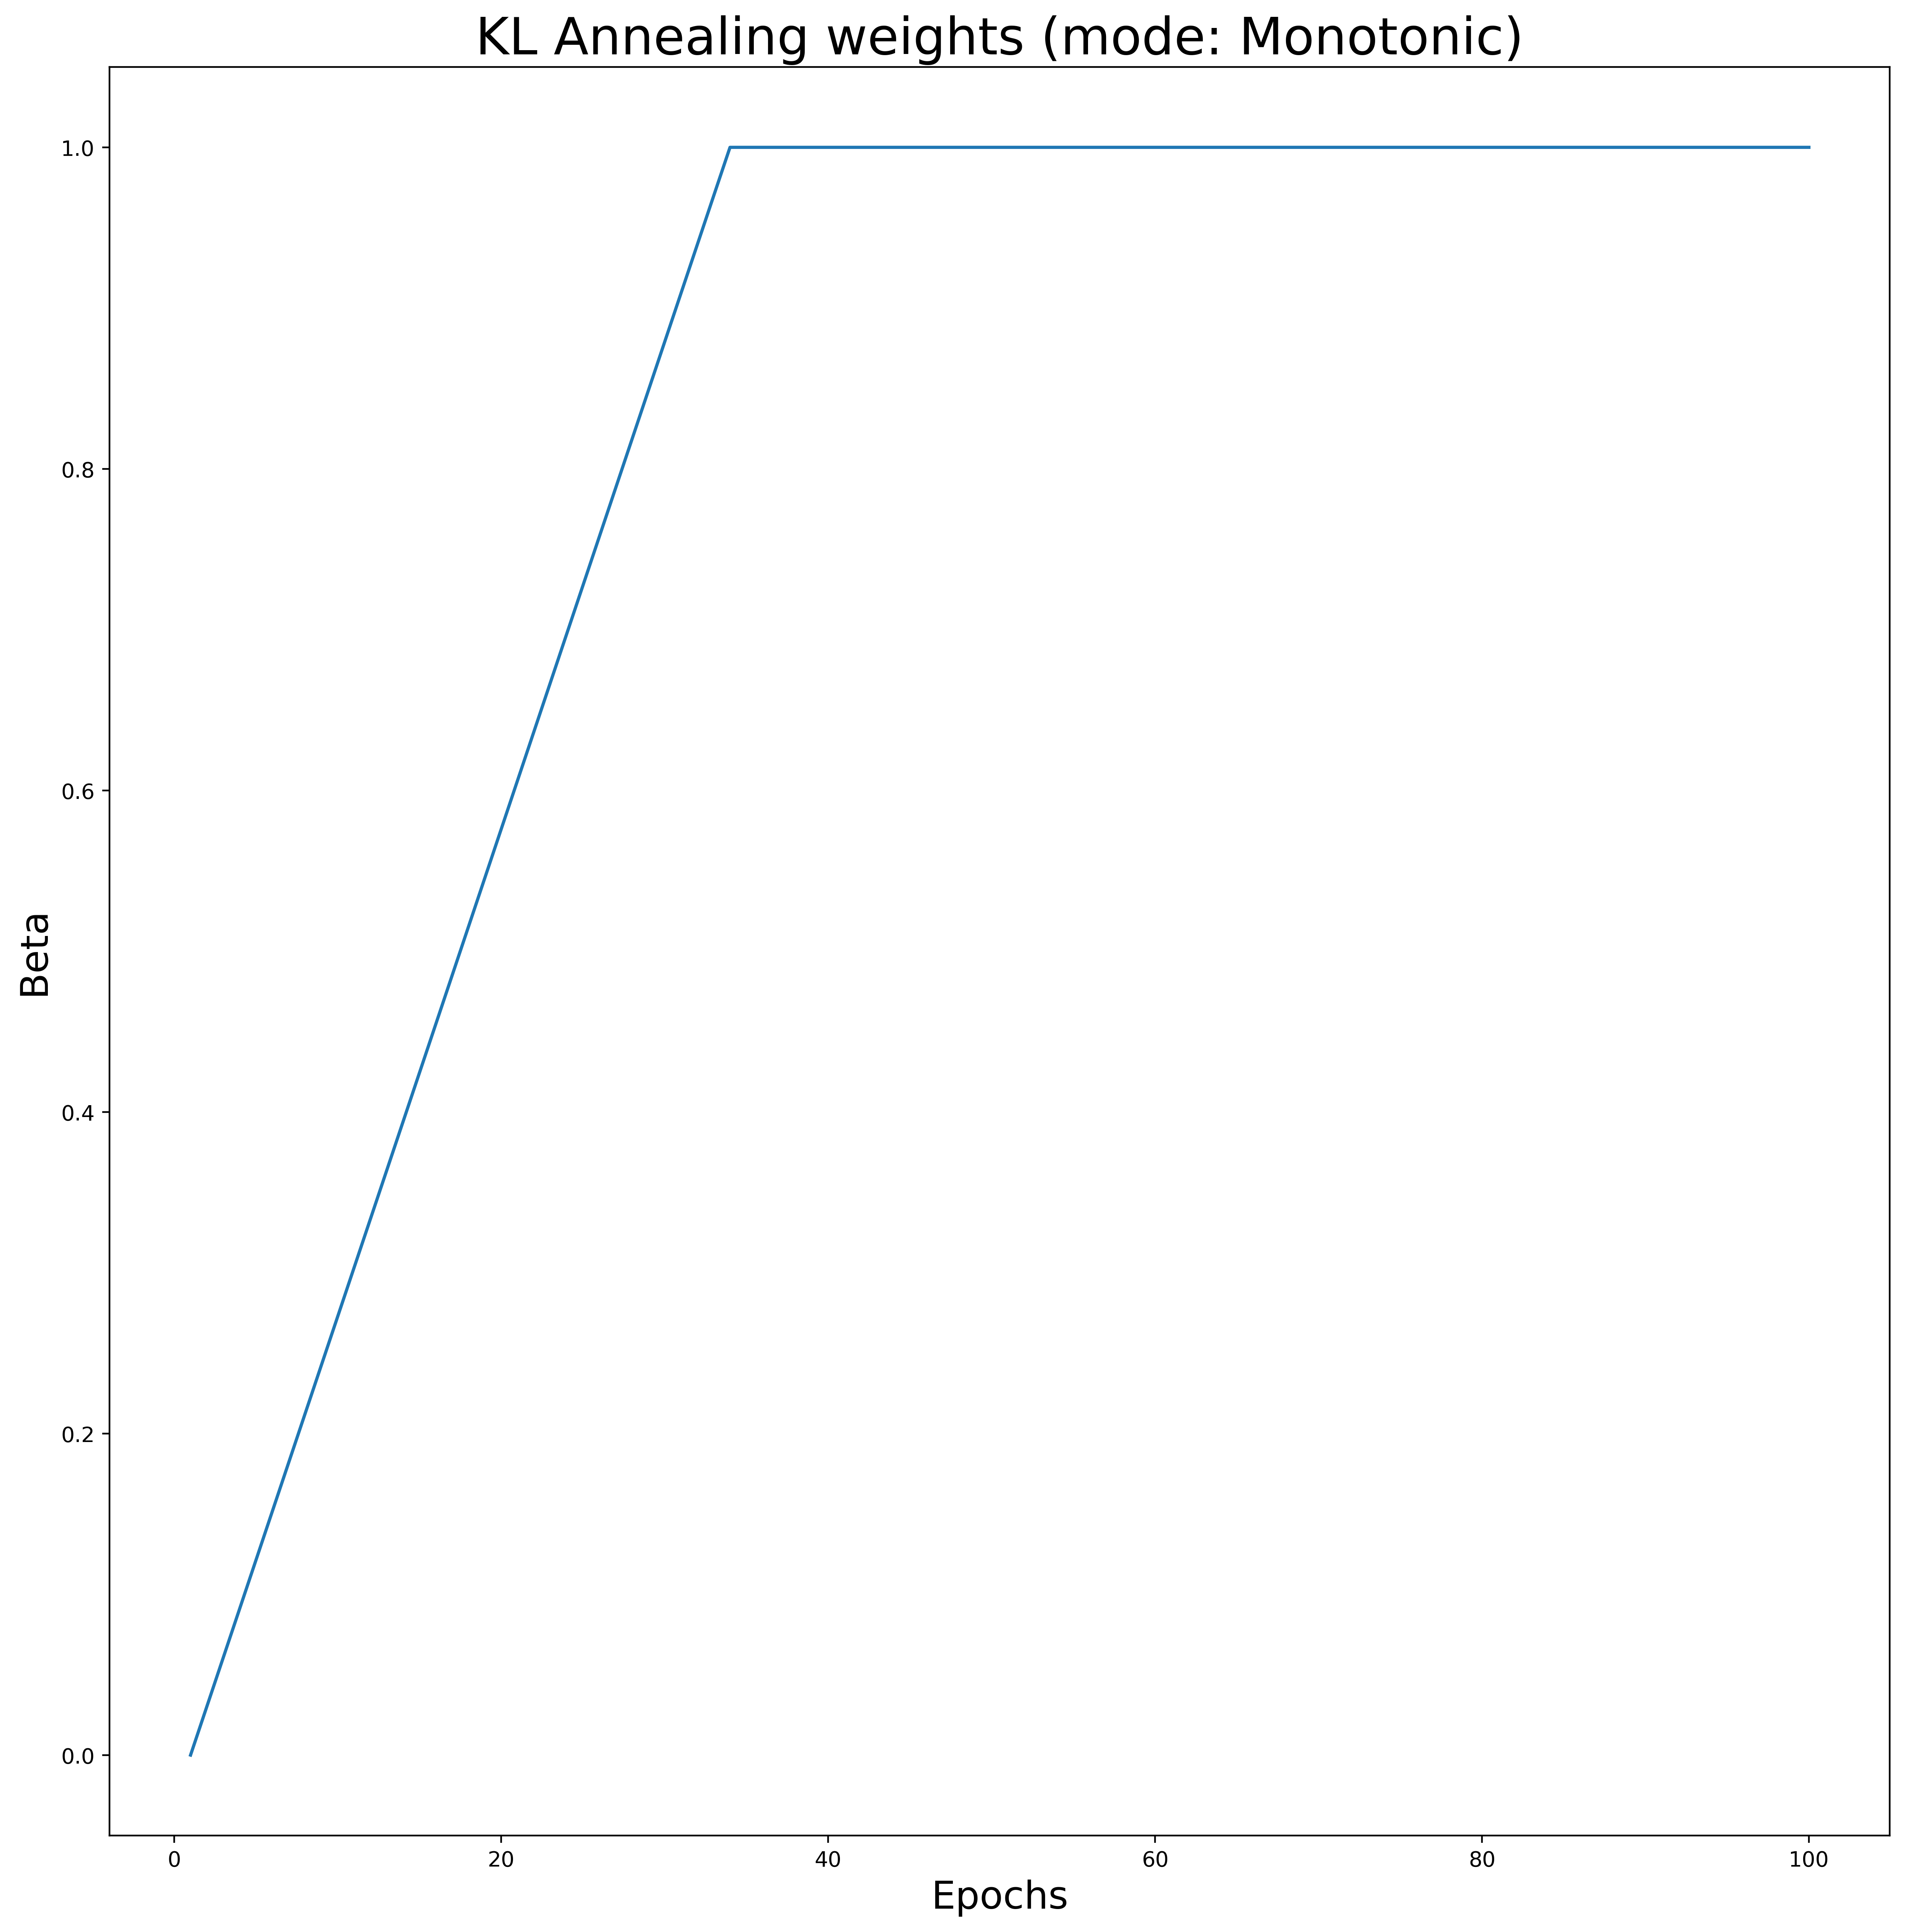
\includegraphics[width=0.45\textwidth]{img/mono.png}
            \label{kl-annealing-mono}
        \end{subfigure}
        \hfill
        \begin{subfigure}
            \centering
            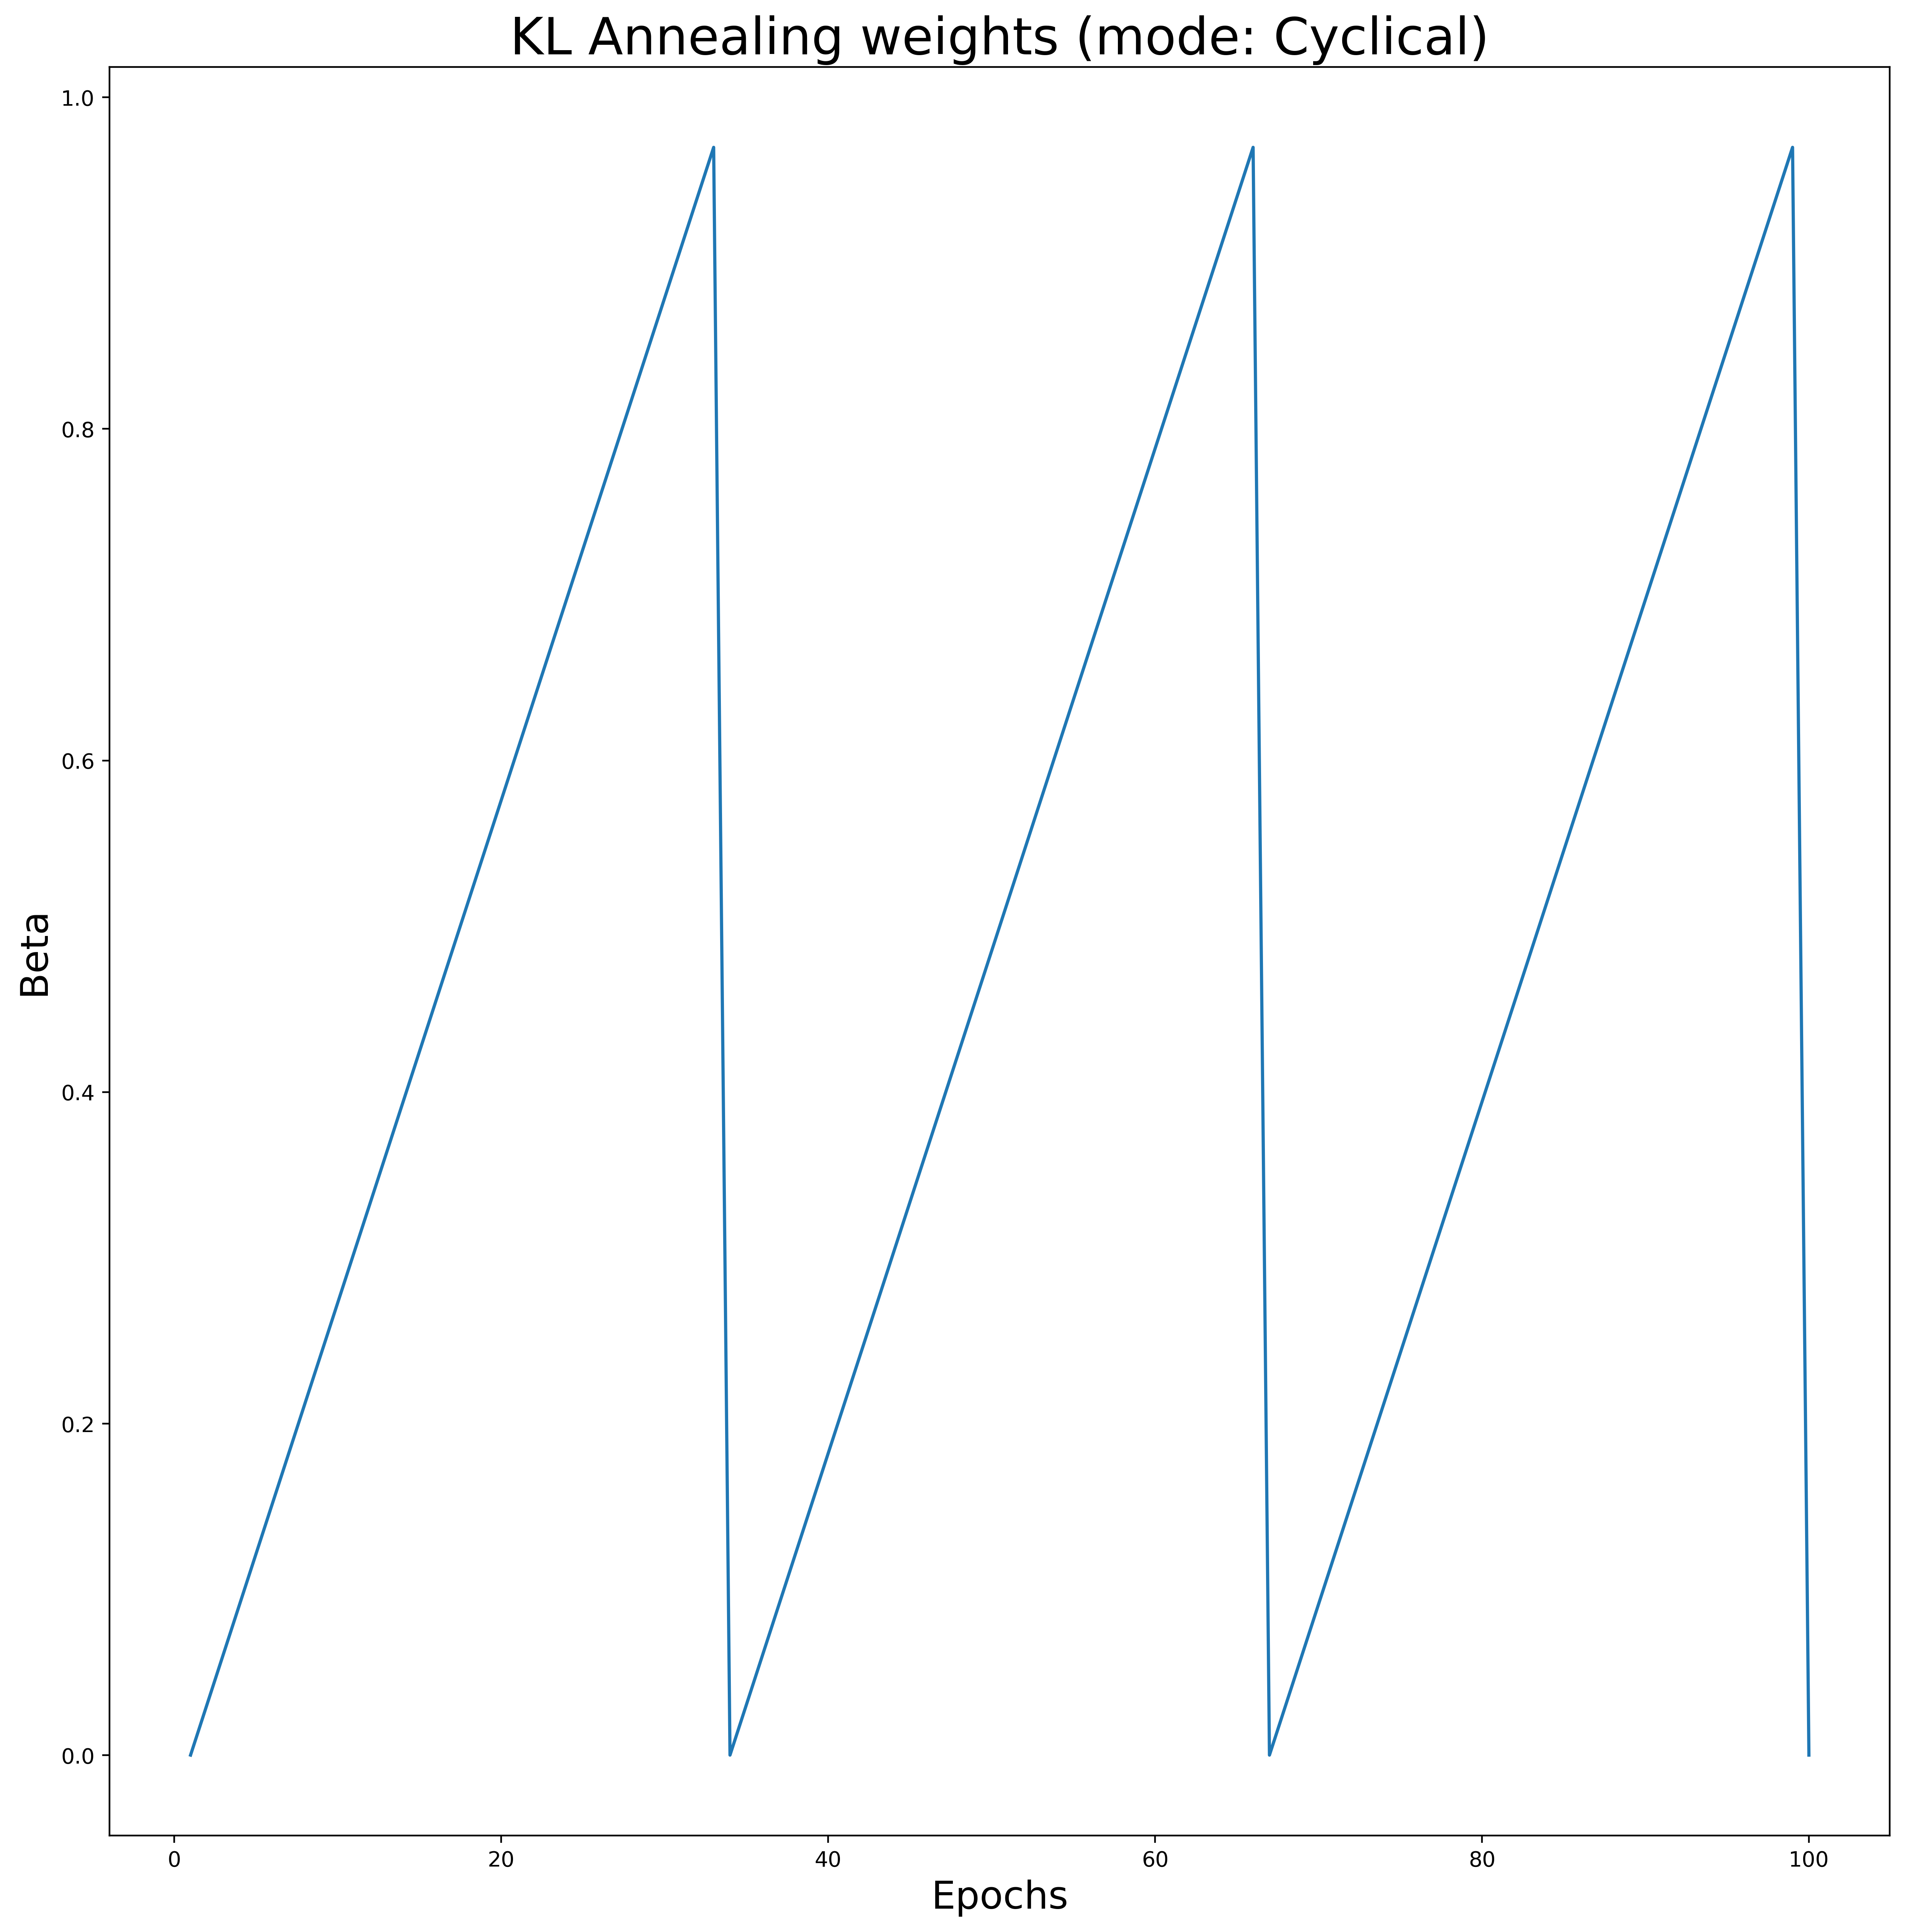
\includegraphics[width=0.45\textwidth]{img/cyc.png}
            \label{kl-annealing-cyc}
        \end{subfigure}
        \hfill
        \caption{Illustration of KL annealing.\\Left sub-figure is monotonic mode, and right is cyclical.}
   \end{figure}

\begin{lstlisting}[language=Python, caption={Python code of \textcolor{blue}{\textbf{KlAnnealing}} (some code is omitted).}, label={kl-annealing}]
class KlAnnealing(object):
    def __init__(self, 
            ratio: float, cycle: int, num_epochs: int, beta_min: float, 
            mode='mono') -> None:
        self.cycle_num_epochs = num_epochs // cycle
        self.step = 1 / (self.cycle_num_epochs * ratio)
        
        self.beta_min = beta_min
        self.epoch = 0
        
        self.__method = self.__monotonic if mode == 'mono' else self.__cyclical
        
    def __monotonic(self) -> float:
        beta = min(self.beta_min + self.epoch * self.step, 1.0)
        
        return beta
    
    def __cyclical(self) -> float:
        beta = min(self.beta_min + (self.epoch % self.cycle_num_epochs) * self.step, 1.0)
            
        return beta
    
    def update(self) -> None:
        self.epoch += 1
    
    @property
    def weight(self) -> float:
        return self.__method()\end{lstlisting}

\section{Teacher-forcing}
\indent
    When teacher-forcing is used, then the input of previous frame is ground-truth.
    This approach can make the model converge faster during early training, 
    since when the predicted previous frame has some error and it's used as input, 
    then the error becomes larger during training.
    However, if we always use teacher-forcing, exposure bias may occur. \\
    The best approach is using scheduled sampling, use teacher-forcing with probability $p$, 
    and gradually decreases $p$ during training (See Listing \ref{teacher-forcing}).

\begin{lstlisting}[language=Python, caption={Python code of \textcolor{blue}{\textbf{Solver}} (some code is omitted).}, label={teacher-forcing}]
for epoch in tqdm(range(self.epoch_start, self.epoch_start + self.num_epochs)): 
    for _ in range(self.num_iters):
        use_teacher_forcing = True if random.random() < self.tf_ratio else False
        seq_pred = seq[:, 0]
        for frame_idx in range(len_seq - 1): 
            input_prev = seq[:, frame_idx]
            
            if use_teacher_forcing: 
                h_prev = self.encoder(input_prev)
            else:
                h_prev = self.encoder(seq_pred)

            if self.is_last_frame_skipped or frame_idx + 1 < self.num_cond:
                h_prev, skip = h_prev
            else:
                h_prev = h_prev[0]

            # Omitted.

            seq_pred = self.decoder([h_pred, skip])

# Omitted.

if epoch >= self.tf_epoch_start_decay: 
    self.tf_ratio = max(
        1 - self.tf_decay_step * (epoch - self.tf_epoch_start_decay), 
        self.tf_ratio_min)
\end{lstlisting}
